% INSERT BEFORE oneb
\pagechapter{1A\quad Class expectations and scientific investigation}{classroom}
\idea{Use the learning targets to guide practice and the evidence to guide your conclusions.}
\subsection*{The assessment system in the class slides}
KUDOS provides the broad overview. The unit guide lists detailed vocabulary and study questions. Classwork, homework, notes, and review prepare students for the unit exams.
\par
\begin{tabularx}{\linewidth}{@{}p{0.26\linewidth}Y@{}}\toprule
Assessment & Supplied class policy\\\midrule
Formative practice & Homework, practice tests, and CFAs give feedback without directly affecting grades.\\
Checkups & 15\% of the grade; cover assigned work. Lowest two per semester dropped. No retake or makeup except for an excused absence.\\
Quality assignments & 20\% of the grade.\\
Quizzes and exams & 45\%. The unit exam can replace the quiz score. Exam retakes are available for scores below 80\%, with homework completion and a retake ticket required.\\
Final exam & 20\% of the grade.\\\bottomrule
\end{tabularx}\par
The slides estimate 15--30 minutes of focused homework nightly. If a student still struggles after more than an hour of focused work, they advise contacting the teacher and seeking tutorial help. These summarize the supplied deck; later teacher announcements may update policies.
\subsection*{Observations become testable explanations}
\begin{center}
\begin{tikzpicture}[concept/.append style={text width=3cm}]
\node[concept] (o) at (0,0) {Observations and data};
\node[concept] (e) at (7.8,0) {General explanation};
\node[concept] (p) at (7.8,-2.1) {Specific prediction};
\node[concept] (t) at (0,-2.1) {Test and compare};
\draw[flow] (o)--node[rel,above]{induction suggests}(e);
\draw[flow] (e)--node[rel,right]{deduction yields}(p);
\draw[flow] (p)--node[rel,below]{guides measurements}(t);
\draw[flow] (t)--node[rel,left]{produces new}(o);
\end{tikzpicture}\par
\end{center}
A \textbf{hypothesis} is a testable proposed explanation. A \textbf{prediction} states a result expected if that explanation applies. Deduction guarantees a conclusion only with a valid argument and true premises; inductive conclusions remain revisable. Science uses both forms.
\textbf{Geotastic example.} A visible road sign is an observation; the inferred country is an interpretation. Comparing guessing error with the number of allowed advances can test a prediction, but player experience and location difficulty may also affect error.
\classsource{Biology Class Basics, slides 3--8; Deductive vs Inductive Reasoning Overview; Observation and Inference; Geotastic Inference Game.}

% INSERT BEFORE onec
\pagechapter{1B\quad The characteristics of life}{lifecheck}
\idea{A living organism is an organized cellular system. No single sign, such as movement or growth, is enough to identify life.}
\par
\begin{tabularx}{\linewidth}{@{}p{0.26\linewidth}Y@{}}\toprule
Characteristic & Meaning and a useful example\\\midrule
Made of cells & Cells are the basic units of life. A bacterium is unicellular; a tree is multicellular.\\
Reproduction & Organisms produce offspring through a life cycle or lineage. A sterile individual can still be alive.\\
Genetic information & DNA stores inherited information; RNA helps cells use that information. Offspring inherit information from parents.\\
Growth and development & Growth increases size or cell number. Development changes form or function, such as a seedling forming mature leaves.\\
Matter and energy use & Metabolic reactions supply materials and usable energy for cellular work. A plant takes in carbon dioxide and captures light energy.\\
Response to stimuli & A stimulus is a change an organism detects. A plant growing toward light is a response; walking is not required.\\
Homeostasis & Organisms regulate internal conditions within functional ranges even while the surroundings change.\\
Evolution & Inherited characteristics of populations change across generations. An individual does not evolve during its lifetime.\\\bottomrule
\end{tabularx}\par
\subsection*{Apply the whole checklist}
\textbf{Fire} spreads, uses fuel, and releases heat, but has no cells or biological genetic system. \textbf{A dormant seed} may show little visible activity, but contains living cells and can resume growth under suitable conditions. \textbf{A sterile mule} is alive despite its inability to reproduce.
\subsection*{Metabolism connects the characteristics}
Building molecules supports growth and repair. Breaking down fuel molecules can transfer energy to ATP. ATP supports movement, synthesis, and transport across membranes. These processes help cells maintain homeostasis.

\textbf{Do not confuse terms.} Metabolism is the collection of chemical reactions; homeostasis is regulation of conditions. Respiration is one metabolic process that helps supply energy for regulation. The class's example of a room warming when people enter connects cellular respiration to heat released into the surroundings.
\memorycheck{Explain why a feather is biologically derived material but is not itself a living organism.}
\classsource{Lecture 1 What Is Life Skeleton Notes; Metabolism, Trophic Levels and Energy Transfer, slides 2 and 5--7.}

\pagechapter{1B\quad Cells and viruses}{cells}
\idea{Viruses share genetic information and evolution with living systems, but lack the independent cellular organization used in the class's life checklist.}
\begin{center}
\begin{tikzpicture}[font=\small\sffamily]
\draw[thick,forest,fill=pale] (0,0) ellipse (2.6 and 1.6);
\draw[blue,thick] plot[smooth] coordinates {(-1,0)(-0.6,0.5)(0,0.1)(0.5,0.6)(1,0.1)(0.6,-0.6)(0,-0.3)(-1,0)};
\foreach \x/\y in {-1.7/0.7,-1.5/-0.8,1.4/0.6,1.6/-0.6,0.3/1.1} {\fill[orange] (\x,\y) circle (0.07);}
\node at (0,2.2) {A simple cell};
\node[align=center] at (0,-2.2) {Membrane, genetic material\\and cellular machinery};
\draw[flow] (3.3,0.7)--(2.45,0.7);
\node[anchor=west] at (3.3,0.7) {membrane};
\begin{scope}[xshift=9.5cm]
\draw[thick,forest,fill=pale] (0,1.2)--(1.1,0.6)--(1.1,-0.6)--(0,-1.2)--(-1.1,-0.6)--(-1.1,0.6)--cycle;
\draw[blue,thick] plot[smooth] coordinates {(-0.6,0.3)(-0.2,0.6)(0.3,0.2)(-0.3,-0.2)(0.3,-0.6)(0.6,-0.2)};
\node at (0,2.2) {A virus particle};
\node[align=center] at (0,-2.2) {Genetic material\\inside a protein coat};
\end{scope}
\end{tikzpicture}\par
\end{center}
\textit{Schematic, not to scale.} The blue line represents genetic material; the cell's orange dots represent ribosomes. Shapes vary, and some viruses also have an envelope.
\par
\begin{tabularx}{\linewidth}{@{}p{0.25\linewidth}Y Y@{}}\toprule
Feature & Cellular organism & Virus\\\midrule
Organization & One or more cells & Not made of cells\\
Genome & DNA & DNA or RNA\\
Metabolism & Has cellular metabolism & Lacks an independent metabolic system\\
Making copies & Uses cellular machinery & Requires a host cell's machinery\\
Evolution & Populations evolve & Viral populations evolve too\\\bottomrule
\end{tabularx}\par
\subsection*{How to answer the classification question}
State the criteria, then apply them. Under the usual school biology criteria, viruses are classified as nonliving because they are not cellular and cannot independently carry out metabolism or make new particles. Their genetic information and capacity to evolve explain why the comparison is interesting.

The viral coat helps protect the genome and, through viral surface structures, enables attachment to suitable host cells. A host cell supplies machinery and resources used to assemble new virus particles. A virus does not simply grow and divide like a cell.
\memorycheck{Why does requiring a host's cellular machinery matter more than simply requiring food from the environment?}
\classsource{Lecture 1 What Is Life Skeleton Notes, virus questions. Verification: \href{https://openstax.org/books/biology-2e/pages/21-introduction}{OpenStax Biology 2e, Viruses}.}

\pagechapter{1B\quad Drawing feedback loops}{feedback}
\idea{Track one measurable condition. Negative feedback opposes its change; positive feedback reinforces it. The sign describes a relationship, not whether a response is helpful.}
\subsection*{Temperature regulation in both directions}
\begin{center}
\begin{tikzpicture}[concept/.append style={text width=3cm}]
\node[concept] (hot) at (0,0) {Temperature rises above its range};
\node[concept] (sweat) at (5.1,0) {Sweating increases};
\node[concept] (down) at (10.2,0) {Temperature decreases};
\draw[flow] (hot)--node[rel,above]{triggers}(sweat);
\draw[flow] (sweat)--node[rel,above]{helps cause}(down);
\draw[flow] (down.south)--++(0,-0.8)-|node[rel,pos=0.25,below]{reduces further sweating}(sweat.south);
\node[concept] (cold) at (0,-3.2) {Temperature falls below its range};
\node[concept] (shiver) at (5.1,-3.2) {Shivering increases};
\node[concept] (up) at (10.2,-3.2) {Temperature increases};
\draw[flow] (cold)--node[rel,above]{triggers}(shiver);
\draw[flow] (shiver)--node[rel,above]{helps cause}(up);
\draw[flow] (up.south)--++(0,-0.8)-|node[rel,pos=0.25,below]{reduces further shivering}(shiver.south);
\end{tikzpicture}\par
\end{center}
Sweat evaporation transfers heat away from the body. Shivering uses repeated muscle contractions; greater energy use and metabolism release more heat. Recovery toward the regulated range reduces corrective action.
\subsection*{A self-reinforcing loop}
\begin{center}
\begin{tikzpicture}[concept/.append style={text width=3cm}]
\node[concept] (p) at (0,0) {Pressure on cervix};
\node[concept] (s) at (5.1,0) {Signals promote oxytocin release};
\node[concept] (c) at (10.2,0) {Stronger uterine contractions};
\draw[flow] (p)--node[rel,above]{triggers}(s);
\draw[flow] (s)--node[rel,above]{stimulates}(c);
\draw[flow] (c.south)--++(0,-0.8)-|node[rel,pos=0.3,below]{increase pressure, repeating the loop}(p.south);
\end{tikzpicture}\par
\end{center}
Delivery removes the initiating pressure. A chain that never returns to affect the original condition is not a complete feedback explanation.
\memorycheck{Choose an everyday condition, draw a response, and show how it changes the same condition.}
\classsource{Feedback Mechanisms and Homeostasis, slides 2--5; Feedback Mechanisms and Homestasis Practice.}

% INSERT BEFORE pyramids
\pagechapter{1C\quad Diagramming energy and gases}{gases}
\idea{Separate energy transfers from gas exchange. Gases enter or leave the surroundings rather than passing along feeding arrows.}
\subsection*{Energy pathway}
\begin{center}
\begin{tikzpicture}[concept/.append style={text width=2.35cm}]
\node[concept] (sun) at (0,0) {Sunlight};
\node[concept] (plant) at (3.7,0) {Producer};
\node[concept] (animal) at (7.4,0) {Consumer};
\node[concept] (decomp) at (11.1,0) {Decomposer};
\draw[flow] (sun)--node[rel,above]{light}(plant);
\draw[flow] (plant)--node[rel,above]{food}(animal);
\draw[flow] (animal)--node[rel,above,text width=1.4cm]{remains\\and waste}(decomp);
\foreach \a in {plant,animal,decomp} {
\draw[-{Stealth},thick,orange] (\a.south)--++(0,-1.1) node[below,font=\scriptsize\sffamily,text width=2.8cm,align=center]{heat to surroundings};
}
\draw[flow,dashed] (plant.north)--++(0,1)-|node[rel,pos=0.3,above]{dead producers also feed decomposers}(decomp.north);
\end{tikzpicture}\par
\end{center}
Photosynthesis converts light to chemical energy. Feeding transfers organic molecules and their chemical energy. Cellular respiration transfers energy to ATP, while metabolic processes release heat. Decomposers receive remains from any trophic level.
\subsection*{Gas exchange with the surroundings}
\begin{center}
\begin{tikzpicture}[concept/.append style={text width=3.2cm}]
\node[concept,fill=blue!6] (co) at (0,0) {Carbon dioxide\\in air};
\node[concept] (photo) at (5.2,0) {Photosynthesis\\in a producer};
\node[concept,fill=blue!6] (ox) at (10.4,0) {Oxygen\\in air};
\draw[flow,blue] (co)--node[rel,above]{taken in}(photo);
\draw[flow,blue] (photo)--node[rel,above]{released}(ox);
\node[concept,fill=blue!6] (ox2) at (0,-2.3) {Oxygen\\in air};
\node[concept] (resp) at (5.2,-2.3) {Aerobic cellular respiration};
\node[concept,fill=blue!6] (co2) at (10.4,-2.3) {Carbon dioxide\\in air};
\draw[flow,blue] (ox2)--node[rel,above]{taken in}(resp);
\draw[flow,blue] (resp)--node[rel,above]{released}(co2);
\end{tikzpicture}\par
\end{center}
The respiration row applies to plants, animals, and aerobic decomposers. Plants need both sets of gas arrows. Aquatic organisms may exchange dissolved gases with water rather than directly with air.
\textbf{Decomposition} acts on dead material; the decomposer uses its own metabolism. Some microbes use pathways without oxygen, so the aerobic row does not represent every microbe.
\memorycheck{Draw a plant, a rabbit, and aerobic decomposers. Add food, heat, and gas arrows for every relevant process.}
\classsource{Metabolism, Trophic Levels and Energy Transfer, slides 2--7 and 19--27; Energy, Ecosystems, and Ecology Part 1; Energy and Matter Language Guide.}

\pagechapter{1C\quad Consumer roles and energy language}{roles}
\idea{Feeding role describes how an organism obtains organic matter. Trophic level describes its position in a particular feeding pathway.}
\par
\begin{tabularx}{\linewidth}{@{}p{0.25\linewidth}Y Y@{}}\toprule
Role & Definition & Example\\\midrule
Herbivore & Eats plants or algae & Rabbit eating grass\\
Carnivore & Eats animals & Hawk eating a rabbit\\
Omnivore & Eats plant and animal material & Bear eating berries and fish\\
Scavenger & Consumes remains of dead animals & Vulture feeding on a carcass\\
Detritivore & Ingests small pieces of dead organic matter & Earthworm eating organic material in soil\\
Decomposer & Breaks down organic matter externally and absorbs products & Fungus growing on dead wood\\\bottomrule
\end{tabularx}\par
These categories can overlap. Detritivores physically process material; microbial decomposers chemically break it down and return nutrients to reusable forms. Decomposers are heterotrophs, not producers.
\subsection*{Trace the molecules and the energy separately}
\textbf{Digestion} breaks food into smaller molecules that can be absorbed. \textbf{Cellular respiration} processes fuel molecules in cells, transferring chemical energy to ATP. \textbf{ATP} provides an immediate energy supply for muscle contraction, molecule synthesis, and transport across membranes.

Plants obtain most of the carbon in their organic molecules from carbon dioxide. Fertilizer supplies mineral nutrients; it does not supply the sunlight captured in photosynthesis. Water and minerals contribute matter, while light supplies energy.

\textbf{Say:} organisms obtain, store, convert, transfer, or release energy. Avoid saying organisms create energy or that glucose simply becomes ATP. During respiration, energy is transferred to ATP while atoms from fuel molecules are rearranged into products.
\subsection*{Worked comparison}
A wood-burning stove and a person both use energy stored in organic matter and release heat. In the person, cellular pathways also transfer energy to ATP for regulated cellular work. The stove does not have cells, homeostasis, or biological reproduction.

Shivering connects the same ideas: muscle contraction uses ATP, metabolism supplies usable energy, and heat release helps raise body temperature. Increased metabolic rate means more reactions per unit time, not the creation of new energy.
\memorycheck{Why is a mushroom a heterotroph even though it never chases prey?}
\classsource{Metabolism, Trophic Levels and Energy Transfer, slides 12--20; Trophic Levels Skeleton Notes; Energy and Matter Language Guide and questions; Energy and Matter Practice Questions.}

\pagechapter{1C\quad The energy-flow lab}{lab}
\idea{Compare water-temperature changes across control, still-hand, and moving-hand conditions, then explain the energy pathway.}
\begin{center}
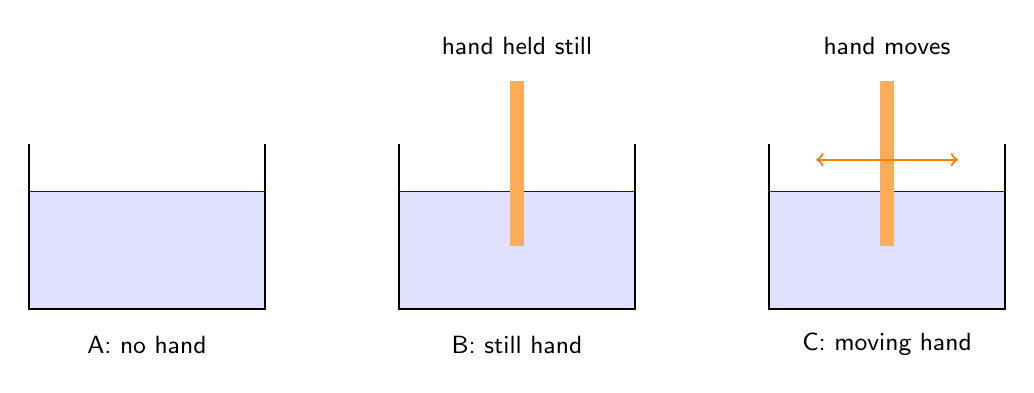
\begin{tikzpicture}[font=\small\sffamily]
\foreach \x/\lab in {0/A: no hand,4.7/B: still hand,9.4/C: moving hand} {
\fill[blue!12] (\x,0) rectangle ++(3,1.5);
\draw[thick] (\x,2.1)--(\x,0)--++(3,0)--++(0,2.1);
\draw[blue] (\x,1.5)--++(3,0);
\node at (\x+1.5,-0.45) {\lab};
}
\draw[line width=5pt,orange!65] (6.2,2.9)--(6.2,0.8);
\draw[line width=5pt,orange!65] (10.9,2.9)--(10.9,0.8);
\draw[<->,thick,orange] (10,1.9)--(11.8,1.9);
\node at (6.2,3.35) {hand held still};
\node at (10.9,3.35) {hand moves};
\end{tikzpicture}\par
\end{center}
\textit{Setup schematic.} Colored bars represent hands, not thermometers. The handout uses a 500-ml bottle of water for each container and records temperature initially and once each minute for five minutes.
\begin{center}
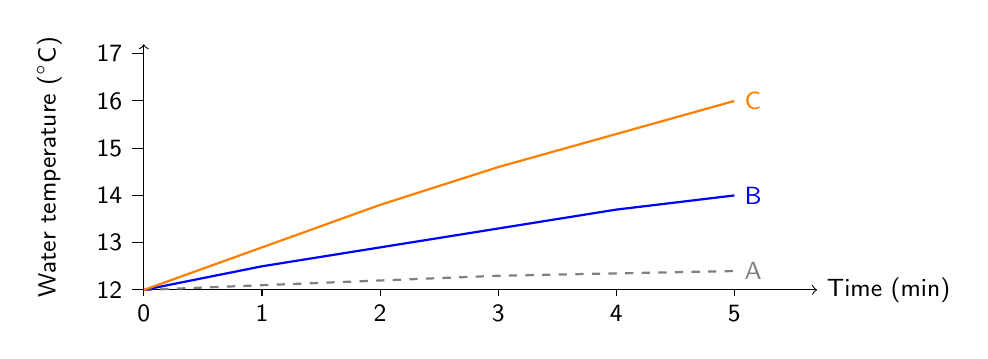
\begin{tikzpicture}[x=1.5cm,y=0.60cm,font=\small\sffamily]
\draw[->] (0,0)--(5.7,0) node[right]{Time (min)};
\draw[->] (0,0)--(0,5.2);
\node[rotate=90] at (-0.8,2.6) {Water temperature ($^\circ$C)};
\foreach \x in {0,1,2,3,4,5} {\draw (\x,0)--(\x,-0.12) node[below]{\x};}
\foreach \y/\lab in {0/12,1/13,2/14,3/15,4/16,5/17} {\draw (0,\y)--(-0.1,\y) node[left]{\lab};}
\draw[gray,thick,dashed] plot coordinates {(0,0)(1,0.1)(2,0.2)(3,0.3)(4,0.35)(5,0.4)} node[right]{A};
\draw[blue,thick] plot coordinates {(0,0)(1,0.5)(2,0.9)(3,1.3)(4,1.7)(5,2)} node[right]{B};
\draw[orange,thick] plot coordinates {(0,0)(1,0.9)(2,1.8)(3,2.6)(4,3.3)(5,4)} node[right]{C};
\end{tikzpicture}\par
\end{center}
\textbf{Invented practice data, not Shawn's results.} Changes are A: $0.4^\circ$C, B: $2.0^\circ$C, C: $4.0^\circ$C. A shows warming possible without a hand. Initial temperatures, hand size, movement, and timing are potential sources of variability.
\textbf{Heat calculation.} The handout's approximation for water is:
\[
Q\;(\mathrm{Cal})=V\;(\mathrm{L})\times\Delta T\;({}^\circ\mathrm C).
\]
For 0.50 L warmed by $4.0^\circ$C, $Q=2.0$ Cal, or 2 kcal. This is heat gained by the water, not all energy used by the body. Movement also affects mixing and heat transfer, so water warming does not isolate metabolic heat production.
\classsource{Energy Flow Lab 2021, procedure and quantitative questions; Energy and Matter Language Guide.}

% INSERT BEFORE twob
\pagechapter{2A\quad Seeing biodiversity at three scales}{diversity}
\idea{Genetic, species, and ecosystem diversity describe different levels. State which level your evidence measures.}
\begin{center}
\begin{tikzpicture}[font=\small\sffamily]
\foreach \x/\title in {0/Genetic diversity,4.7/Species diversity,9.4/Ecosystem diversity} {
\draw[forest,rounded corners] (\x,0) rectangle ++(4,3);
\node at (\x+2,3.4) {\title};
}
\foreach \x/\y/\lab in {0.7/0.8/A,2/0.8/a,3.2/0.8/A,0.7/2/a,2/2/A,3.2/2/a} {
\draw[forest,fill=pale] (\x,\y) circle (0.32);
\node at (\x,\y) {\lab};
}
\foreach \x/\y in {5.4/0.8,6.5/2,7.8/0.8} {\draw[forest,fill=pale] (\x,\y) circle (0.25);}
\foreach \x/\y in {5.4/2,6.6/0.8,7.8/2} {\draw[blue,fill=blue!10] (\x-0.25,\y-0.25) rectangle ++(0.5,0.5);}
\fill[forest!30] (9.7,1.6) rectangle ++(1.5,1);
\fill[blue!20] (11.4,1.6) rectangle ++(1.6,1);
\fill[orange!20] (9.7,0.4) rectangle ++(3.3,0.9);
\node[font=\scriptsize\sffamily] at (10.45,2.1) {forest};
\node[font=\scriptsize\sffamily] at (12.2,2.1) {wetland};
\node[font=\scriptsize\sffamily] at (11.35,0.85) {grassland};
\node[align=center,text width=4cm] at (2,-0.85) {Same species,\\different alleles};
\node[align=center,text width=4cm] at (6.7,-0.85) {Different symbols\\represent different species};
\node[align=center,text width=4cm] at (11.4,-0.85) {Different habitats and\\ecological communities};
\end{tikzpicture}\par
\end{center}
Letters represent schematic alleles, not complete genotypes. Genetic variation can increase the chance that some individuals tolerate a change. It cannot guarantee that a helpful trait exists or that every individual survives.
\subsection*{Why species roles matter}
A \textbf{keystone species} has an unusually large effect relative to its abundance. Some predators regulate prey and thereby influence vegetation and other organisms. The effect depends on the food web; not every predator is a keystone species.

The worksheet asks why corals matter. Reef-building corals create physical habitat used for shelter and feeding. Losing reef structure can affect many species. This habitat-building role is often described more precisely as a \textbf{foundation species} role.
\begin{center}
\begin{tikzpicture}[concept/.append style={text width=3cm}]
\node[concept] (c) at (0,0) {Reef-building corals};
\node[concept] (h) at (5.1,0) {Complex reef habitat};
\node[concept] (f) at (10.2,0) {Fish and invertebrate communities};
\draw[flow] (c)--node[rel,above]{build}(h);
\draw[flow] (h)--node[rel,above]{supports}(f);
\end{tikzpicture}\par
\end{center}
\textbf{Services connect mechanisms to people.} Fish are provisioning resources; water purification is regulating; nutrient cycling is supporting; recreation and cultural meaning are cultural benefits. Explain both the category and the process.
\memorycheck{Does a forest with many trees, all of one species, necessarily have high tree species diversity?}
\classsource{Biodiversity Worksheet; Biodiversity and Its Threats Debrief, slides 2--6. Coral clarification: \href{https://coralreef.noaa.gov/digital-corals/visual-media/infographics/corals-are-important}{NOAA, Corals are Important}.}

% INSERT BEFORE cer
\pagechapter{2B\quad Habitat loss and corridors}{habitat}
\idea{Habitat amount and connectivity are different. Protecting one does not automatically protect the other.}
\begin{center}
\begin{tikzpicture}[font=\small\sffamily]
\foreach \x/\title in {0/Connected habitat,4.7/Divided by a road,9.4/With a crossing} {
\fill[forest!16] (\x,0) rectangle ++(4,3.5);
\draw[forest] (\x,0) rectangle ++(4,3.5);
\node at (\x+2,4) {\title};
}
\foreach \x in {4.7,9.4} {
\fill[gray!60] (\x+1.6,0) rectangle ++(0.8,3.5);
\draw[white,dashed,thick] (\x+2,0)--++(0,3.5);
}
\fill[forest!50] (10.7,1.35) rectangle (12.1,2.15);
\draw[forest,thick] (10.7,1.35) rectangle (12.1,2.15);
\foreach \x in {0.8,3.1,5.5,7.8,10.2,12.5} {
\fill[orange] (\x,0.8) circle (0.10);
\fill[orange] (\x,2.6) circle (0.10);
}
\draw[<->,thick,forest] (0.8,1.75)--(3.1,1.75);
\draw[<->,thick,forest] (10.2,1.75)--(12.5,1.75);
\node[align=center,text width=4cm] at (2,-0.75) {Movement within\\a continuous area};
\node[align=center,text width=4cm] at (6.7,-0.75) {Habitat removed;\\patches isolated};
\node[align=center,text width=4cm] at (11.4,-0.75) {A route reconnects\\remaining patches};
\end{tikzpicture}\par
\end{center}
\textit{Conceptual landscape, not a measured map.} Dots represent individuals; arrows represent potential movement. Crossings help only if organisms can use them safely.
\subsection*{Four mechanisms}
\begin{enumerate}
\item \textbf{Loss:} development removes feeding and breeding sites. Resource supply and carrying capacity can decrease.
\item \textbf{Isolation:} individuals may struggle to find mates or recolonize a patch. Reduced gene flow can compound the problem over generations.
\item \textbf{Edge effects:} temperature, moisture, predators, and human disturbance may differ near habitat boundaries.
\item \textbf{Connectivity:} a suitable corridor can support migration, mating, and movement toward newly suitable habitat as conditions change.
\end{enumerate}
Protecting large areas and restoring degraded habitat support resource availability. Corridors support movement. A crossing does not eliminate every road hazard or replace all habitat removed by development.
\subsection*{CHIPPO threats can interact}
A road can remove habitat, introduce pollutants, and provide a route for introduced species. Climate change may further reduce the suitability of isolated patches. Identify the interacting mechanisms instead of assigning one label and stopping.
\memorycheck{A corridor increases immigration into one patch. Does that prove the total regional population grew?}
\classsource{Biodiversity Worksheet; Threats to Biodiversity Notes; Ecology 2 framework, page 1.}

% INSERT BEFORE humans
\pagechapter{2C\quad When carrying capacity changes}{changingk}
\idea{Environmental capacity and actual population size can change at different times. Lower resources do not instantly remove all individuals above a new limit.}
\begin{center}
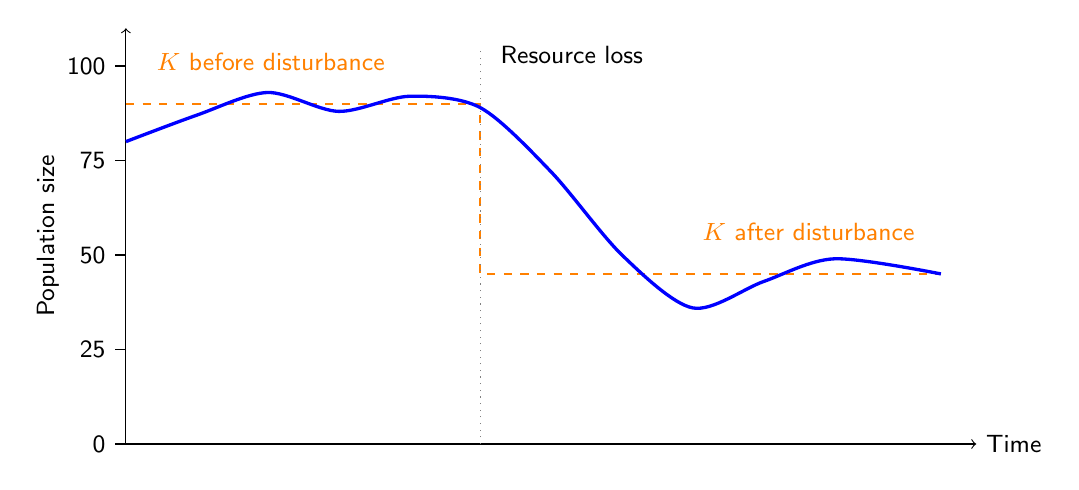
\begin{tikzpicture}[x=0.9cm,y=0.048cm,font=\small\sffamily]
\draw[->] (0,0)--(12,0) node[right]{Time};
\draw[->] (0,0)--(0,110);
\node[rotate=90] at (-1.1,55) {Population size};
\foreach \y in {0,25,50,75,100} {\draw (0,\y)--(-0.15,\y) node[left]{\y};}
\draw[orange,thick,dashed] (0,90)--(5,90)--(5,45)--(11.5,45);
\draw[blue,very thick] plot[smooth] coordinates {(0,80)(1,87)(2,93)(3,88)(4,92)(5,89)(6,72)(7,50)(8,36)(9,43)(10,49)(11.5,45)};
\draw[gray,dotted] (5,0)--(5,105);
\node[anchor=west,text=orange] at (0.3,101) {$K$ before disturbance};
\node[anchor=west,text=orange] at (8,56) {$K$ after disturbance};
\node[anchor=west] at (5.15,103) {Resource loss};
\end{tikzpicture}\par
\end{center}
\textit{Invented illustration.} Orange dashes show $K$; blue shows population size. Values illustrate a pattern, not observations of a particular species.
\subsection*{Interpret the sequence}
Resource loss lowers $K$. The population initially remains above the new capacity, then responds through changes in births, deaths, and movement. Delays and environmental variation can produce later fluctuations.
\begin{center}
\begin{tikzpicture}[concept/.append style={text width=3cm}]
\node[concept] (n) at (0,0) {More individuals\\share finite resources};
\node[concept] (r) at (7.8,0) {Less resource\\per individual};
\node[concept] (b) at (7.8,-2.2) {Births decrease or\\deaths increase};
\node[concept] (g) at (0,-2.2) {Population growth\\slows or reverses};
\draw[flow] (n)--node[rel,above]{can mean}(r);
\draw[flow] (r)--node[rel,right]{can cause}(b);
\draw[flow] (b)--node[rel,below]{so}(g);
\draw[flow] (g)--node[rel,left,text width=2cm]{reduces future\\crowding}(n);
\end{tikzpicture}\par
\end{center}
\textbf{Size} is a count. \textbf{Density} is individuals per area or volume. \textbf{Dispersion} is their spacing, such as clustered, uniform, or random. \textbf{Demography} includes age structure and patterns of births and deaths. These measurements answer different questions.
\memorycheck{After a wildfire, distinguish immediate mortality from a reduction in the number of organisms the remaining habitat can sustain.}
\classsource{Population Ecology KJ, slides 2--14; Population Ecology Skeleton Notes; Ecology 2 framework, page 2.}

% INSERT BEFORE vocab
\pagechapter{2C\quad Resource demand and environmental justice}{resources}
\idea{Human carrying capacity depends on how resources are used and shared, not just on the number of people.}
\subsection*{Understand the Overshoot Day comparison}
Earth Overshoot Day compares annual ecological demand with annual biological regeneration. In the accounting framework:
\[
\text{day of year}\approx
\frac{\text{annual biocapacity}}{\text{annual ecological footprint}}
\times\text{days in the year}.
\]
\textbf{Hypothetical example.} If annual demand is twice annual biocapacity, the ratio is $1/2$. In a 365-day year, the corresponding date is around day 183. Reducing demand to $1.5$ times capacity moves the comparison to about day 243. These are illustrations, not actual annual dates.
\subsection*{What continued overshoot means}
The population slides describe using resources accumulated in the past, reducing resources available to other organisms and people in the present, and limiting future options. Examples include drawing down slowly replenished groundwater, removing old forests, and using fossil fuels. These examples explain resource pressure; Overshoot Day does not directly measure every resource stock.

\textbf{Biocapacity} is productive capacity, while \textbf{ecological footprint} measures demand in a specified accounting system. A date change can reflect demand, biocapacity, or revised estimates. It cannot by itself establish a particular number of species lost.
\subsection*{Quality of life and fairness}
A higher quality of life does not always require proportionally more resources. Less food waste, efficient buildings, and effective public services can deliver benefits with less input. Technology can improve efficiency, but environmental damage and rebound in consumption can offset gains.

Environmental justice asks who receives the benefits, who experiences pollution or scarcity, and who participates in decisions. A strategy that lowers total consumption can still distribute costs unfairly. Evaluate the ecological mechanism and the distribution of consequences.
\subsection*{Explain a solution with a causal chain}
Reducing food waste can reduce demand for crops, land, water, and energy while maintaining nutrition. Habitat restoration can improve productive capacity and biodiversity. Neither example guarantees a particular global date shift; the outcome depends on scale and other changes.
\memorycheck{Explain why increasing resource extraction now can support short-term consumption while lowering future carrying capacity.}
\classsource{Population Ecology KJ, slides 17--19; Ecology 2 framework, page 2. Formula: \href{https://overshoot.footprintnetwork.org/about-earth-overshoot-day/}{Global Footprint Network}.}

% INSERT BEFORE answersone
\pagechapter{Diagram review\quad Applying the class material}{diagrampractice}
These are original review questions based on the supplied class tasks. Draw and explain your answers before checking the answer guide.
\begin{enumerate}
\item \textbf{Cell and virus.} Label a cell membrane, genome, and cellular machinery. Draw a virus beside it and apply the life checklist.
\item \textbf{Feedback.} Draw both branches of temperature regulation. Label condition, response, resulting change, and reduced corrective action.
\item \textbf{Gas and energy.} Draw sunlight, a plant, a rabbit, and aerobic decomposers. Add heat arrows for all living groups and the correct gas arrows to the surroundings.
\item \textbf{Lab.} In invented data, 0.50 L of water warms by $3.0^\circ$C. Estimate heat gained in Calories. Explain the purpose of the no-hand control.
\item \textbf{Biodiversity.} Illustrate variation within one species and variation among species. Explain why the pictures represent different levels.
\item \textbf{Corridor.} Draw a habitat divided by a road and a crossing. Explain effects on movement, gene flow, and habitat amount.
\item \textbf{Changing capacity.} Lower $K$ after a disturbance and draw a delayed population response. Explain the mechanisms.
\item \textbf{CER.} Use actual lab data if available to write a temperature-comparison claim. Separate measured warming from the proposed metabolic explanation.
\item \textbf{Life.} Compare a dormant seed, a fire, and a sterile animal using at least three characteristics.
\item \textbf{Energy.} Explain how digestion, cellular respiration, ATP, and homeostasis are related without saying that matter becomes energy.
\item \textbf{Resources.} If hypothetical demand is 1.25 times annual biocapacity, estimate the corresponding day in a 365-day year. Explain what that comparison does and does not measure.
\item \textbf{Conservation.} A habitat corridor increases movement, but pollution remains. Explain why population recovery is not guaranteed.
\end{enumerate}
\textbf{Diagram checklist.} Label axes and units. Distinguish real data from schematics. Give each arrow a clear meaning and each causal connection a mechanism.

% INSERT BEFORE keynotes
\pagechapter{Diagram review\quad Answer guide}{diagramanswers}
\begin{enumerate}[itemsep=5pt]
\item Cells have membranes and metabolic machinery. Viruses contain a genome and coat but require a host cell to assemble new particles. Shared genetic information alone does not establish cellular life.
\item Warming triggers cooling; cooling reduces the need for further cooling. Falling temperature triggers warming; recovery reduces warming responses. Both oppose the initiating change.
\item Light reaches the plant. Organic molecules move along feeding and decomposition pathways. Every living group releases heat. Photosynthesis takes in carbon dioxide and releases oxygen; aerobic respiration reverses these gas directions. Plants need both sets of arrows.
\item $Q=0.50\times3.0=1.5$ Cal, or 1.5 kcal. The control measures changes possible without a hand. Water heating does not capture all energy used by the body.
\item Allelic differences within a species illustrate genetic diversity; different species illustrate species diversity. Individual counts alone establish neither.
\item A usable crossing can support movement, mating, and recolonization without restoring all removed habitat. Movement into a patch may be redistribution rather than regional growth.
\item Actual numbers can initially exceed the new $K$. Reduced births, increased deaths, or emigration can follow. Exact rates require evidence.
\item Cite actual temperatures and elapsed time. Muscle work uses ATP, metabolism supplies usable energy, and heat transfers to the water. Mixing, hand differences, and starting conditions also affect the measured change.
\item The seed has living cells and genetic information despite dormancy. Fire lacks cells and a biological inheritance system. A sterile animal has cellular organization and metabolism despite reproductive inability.
\item Digestion prepares molecules for absorption. Respiration transfers fuel energy to ATP; ATP supports work needed for homeostasis. Atoms are rearranged, and heat is released.
\item $365/1.25=292$: approximately day 292. This illustrates demand relative to regeneration, not the day all resources physically disappear.
\item Pollution can still reduce survival or reproduction. Connectivity addresses one mechanism; recovery also depends on habitat quality and other limiting factors.
\end{enumerate}
\classsource{Original questions and answers based on the class materials cited in the corresponding chapters.}
